% Paper 2015
\documentclass[11pt,a4paper]{IEEEtran}

% *** MISC UTILITY PACKAGES ***
%
\usepackage{ifpdf}
% Heiko Oberdiek's ifpdf.sty is very useful if you need conditional
% compilation based on whether the output is pdf or dvi.
% usage:
% \ifpdf
   % pdf code
 %\else
   % dvi code
% \fi

% *** CITATION PACKAGES ***
%
\usepackage{cite}

% *** GRAPHICS RELATED PACKAGES ***
%
\ifCLASSINFOpdf
   \usepackage[pdftex]{graphicx}
  % declare the path(s) where your graphic files are
   \graphicspath{{../pdf/}{../jpeg/}}
  % and their extensions so you won't have to specify these with
  % every instance of \includegraphics
   \DeclareGraphicsExtensions{.pdf,.jpeg,.png}
\else
  % or other class option (dvipsone, dvipdf, if not using dvips). graphicx
  % will default to the driver specified in the system graphics.cfg if no
  % driver is specified.
   \usepackage[dvips]{graphicx}
  % declare the path(s) where your graphic files are
  \graphicspath{{../eps/}}
  % and their extensions so you won't have to specify these with
  % every instance of \includegraphics
   \DeclareGraphicsExtensions{.eps}
\fi

% *** MATH PACKAGES ***
%
\usepackage[cmex10]{amsmath}

% *** SPECIALIZED LIST PACKAGES ***
%
\usepackage{algorithmic}

% *** ALIGNMENT PACKAGES ***
%
\usepackage{array}


% *** SUBFIGURE PACKAGES ***
\ifCLASSOPTIONcompsoc
  \usepackage[caption=false,font=normalsize,labelfont=sf,textfont=sf]{subfig}
\else
  \usepackage[caption=false,font=footnotesize]{subfig}
\fi

% *** FLOAT PACKAGES ***
%
\usepackage{fixltx2e}

\usepackage{stfloats}

\ifCLASSOPTIONcaptionsoff
  \usepackage[nomarkers]{endfloat}
 \let\MYoriglatexcaption\caption
\renewcommand{\caption}[2][\relax]{\MYoriglatexcaption[#2]{#2}}
\fi

% *** PDF, URL AND HYPERLINK PACKAGES ***
%
\usepackage{url}

\usepackage{siunitx}
\DeclareSIUnit\photon{\ensuremath{\gamma}}
\DeclareSIUnit\proton{p}
\DeclareSIUnit\neutron{n}

\usepackage{booktabs}
\usepackage{graphicx}
\usepackage{epstopdf}
\usepackage{subfig}

\usepackage{todo}

\usepackage{bpchem}
\def\U238{\BPChem{\^{238}U}}

% correct bad hyphenation here
\hyphenation{op-tical net-works semi-conduc-tor}


\begin{document}
%----------------------------------------------------------------------------------------
%	TITLE SECTION
%----------------------------------------------------------------------------------------
\title{Monte Carlo calculation to characterize neutron and gamma fields for ANITA neutron facility at TSL}

\author{Q. Hong,
S. P. Platt,
A. V. Prokofiev,
E. Passoth
\thanks{further information}\\[2mm] 	% Your name
%\normalsize University of Central Lancashire \\ 							% Your institution
%\normalsize \href{qhong@uclan.ac.uk} 								% Your email address
\vspace{-5mm}
}


%----------------------------------------------------------------------------------------

\maketitle % Insert title
\todo{Check title, affiliations etc.}
%----------------------------------------------------------------------------------------
%	ABSTRACT
%----------------------------------------------------------------------------------------

\begin{abstract}
Monte Carlo simulation of spallation neutron source of ANITA at TSL was used to analyze radiation fields at the Close User Position (CUP) and Standard User Position(SUP) for single-event effect testing. ...\todo{Revise abstract}
\end{abstract}

%----------------------------------------------------------------------------------------
%	KEYWORDS
%----------------------------------------------------------------------------------------


%----------------------------------------------------------------------------------------
%	ARTICLE CONTENTS
%----------------------------------------------------------------------------------------

\IEEEpeerreviewmaketitle

\section{Introduction}
\todo{Review introduction}
\IEEEPARstart{M}{onte} Carlo simulations of naked spallation neutron sources at Los Alamos Neutron Science Center (LANSCE) Weapons Neutron Research (WNR) Target 4\cite{Wender87} and the ANITA beam at the University of Uppsala The Svedberg Laboratory (TSL) have been completed using Geant4 and proved that Binary intranuclear cascade (INC) model gave a good representation of neutron spectra than Bertini INC model did\cite{Platt13}. Simulation result of neutron spectra using Geant4 with Binary INC model is below measurement data from ANITA neutron facility. It is likely to be influenced by our omission of collimator, shielding, and bending magnet component. This work is to verify this hypothesis is correct. In addition, we are intested in the gamma field at CUP and SUP in spallation neutron source at the ANITA neutron facility at TSL for SEE testing.
%------------------------------------------------

\section{Modelling}

A detailed model of the ANITA geometry was implemented in Geant4.
This is illustrated in overview in Fig.~\ref{fig:ANITAoverview}
Description of the geometry is given in \cite{Prokofiev2009,Prokofiev14}; a summary only is given here.
The spallation target is a tungsten cylinder of diameter \SI{5}{\cm} and length \SI{2.4}{\cm}.
The target is cooled by water and surrounded by a stainless-steel cooling jacket.
The target assembly with its cooling jacket appears as a small blue rectangle in Fig.~\ref{fig:ANITAoverview}.
Lead shielding blocks in the target region are also modelled, and shown in red Fig.~\ref{fig:ANITAoverview}.
A large electromagnet surrounding the target is modelled and shown in Fig.~\ref{fig:ANITAoverview} in grey (iron) and yellow (copper).
An iron collimator with variable apertures is modelled  and shown downstream of the target (grey).
For brevity in this summary we only present results for the standard collimator size (\SI{10.2}{\cm} diameter); in the final paper we will present results for cylindrical collimators in the range from \SIrange{3}{30}{\cm} diameter.

\begin{figure}[!t]
	\centering
	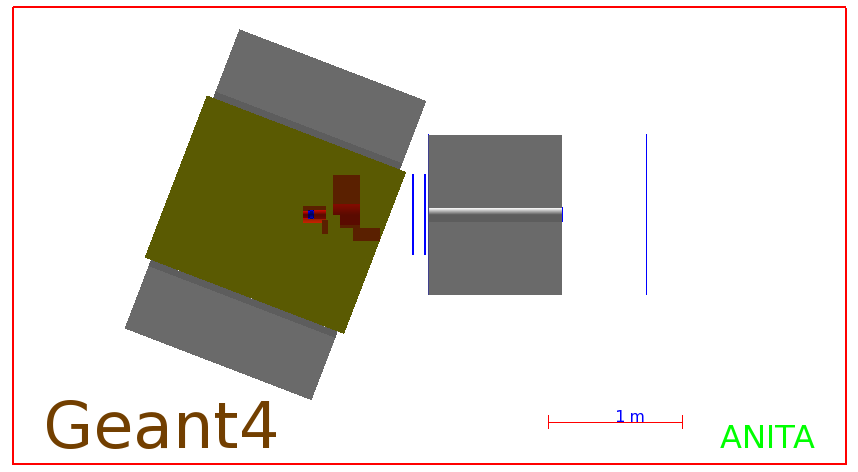
\includegraphics[width=3in]{overview.png}
	\caption{Simulated ANITA facility overview seen from above (yellow: bending magnet; red: shielding components; blue: target cooling jacket (enclosing the target); grey: collimator; blue: detector system)}
	\label{fig:ANITAoverview}
\end{figure}

Simulations were conducted using Geant4 version 10.0.
The binary intranuclear cascade model was selected in accordance with the results of earlier work~\cite{Platt13}, in which it performed well in simulations of neutron spallation in the region from \SIrange{0}{0}{\MeV}.\todo{Enter neutron energy range}
In the simulation protons were incident axially at an energy of \SI{180}{\MeV}.
Resulting gamma and neutron fields were evaluated at several locations.
In this paper results are presented for three of these: The Standard User Position (SUP), \SI{2.5}{\m} downstream of the target centre\todo{check centre}~\cite{Prokofiev2009}, the Close User Position (CUP), \SI{0.75}{\m} downstream of the target, and the CUP-TOF, \SI{0.84}{m} downstream of the target.\todo{Enter CUP \& CUP-TOF ranges}
The SUP, CUP and CUP-TOF positions are visible in blue in Fig.~\ref{fig:ANITAoverview}.
The SUP and CUP positions are of interest as they are positions used for SEE tests; the CUP-TOF position is the location of thin-film breakdown counter (TFBC) detectors used for beam monitoring and characterisation using time-of-flight (TOF) techniques.
Model validation will be demonstrated against CUP-TOF data (section~\ref{tbd}).

%------------------------------------------------
\section{Results}

In previous work Platt et al.~\cite{Platt13} reported simulations of a naked ANITA target, demonstrating good qualitative agreement with independent calculations and measurements of the fast neutron field at ANITA SUP~\cite{Prokofiev2009}.
Part of the motivation for this work was to investigate whether improvements in the fidelity of the geometry used in the Geant4 model would lead to increased quantitative agreement.\todo{Review first part of Results section -- move to introduction?}

\subsection{Neutron fluence rate, spatial distribution and spectrum}

Fig.~\ref{fig:SUPDensity} shows neutron spatial distribution at the SUP.
The collimation effect is clearly visible.
Fig.~\ref{fig:SUPProfile} compares simulated and measured neutron fluence profile at the SUP.
Measurements were taken with a TFBC in which \U238\ is the target material~\cite{Prokofiev2009}; accordingly, simulated results were folded in energy with the neutron fission cross section for \U238~\cite{tbd}.
The results show~\todo{Explain SUP profile results. Include explanation of ``umbra'' and ``penumbra''}
The predicted neutron fluence rate above \SI{10}{\MeV} at a proton current of \SI{200}{\nA} is \SI{0}{\neutron\per\cm\squared\per\second}, compared to \SI{0}{\neutron\per\cm\squared\per\second} from earlier calculations~\cite{Platt13} and \SI{0}{\neutron\per\cm\squared\per\second} from the parameterisation~\cite{Prokofiev2009}.
The parameterisation therefore exceeds the current calculations by tbd\%.\todo{Quantify integral yield}

\begin{figure}[t]
%    \vspace{2in}
    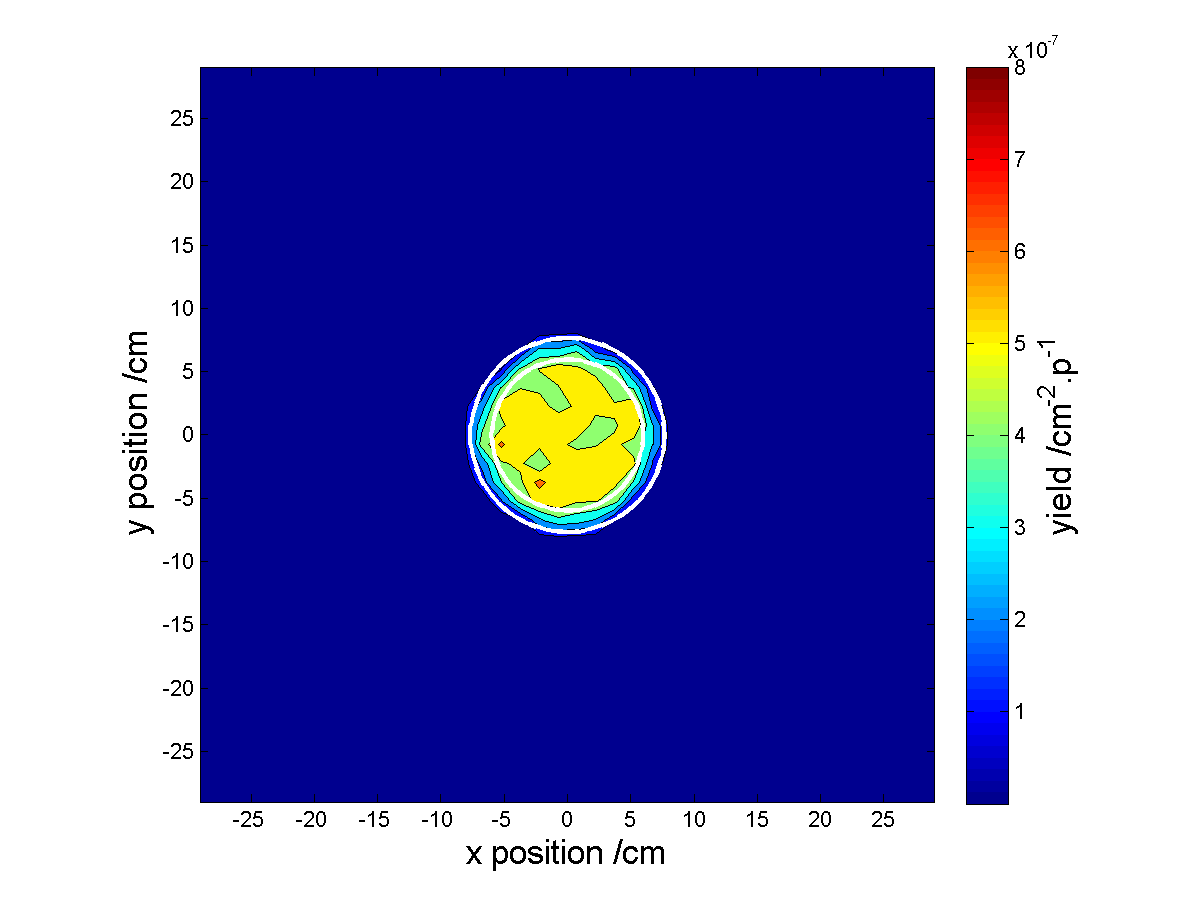
\includegraphics[width=3in]{SUP10ColSpatialDistribution10MeVRADECS.png}
% \todo{Show density of neutrons above \SI{10}{\MeV} at SUP}
    \caption{Neutron fluence rate above \SI{10}{\MeV} at the Standard User Position.}
    \label{fig:SUPDensity}
\end{figure}

\begin{figure}[t]
%    \vspace{2in}
    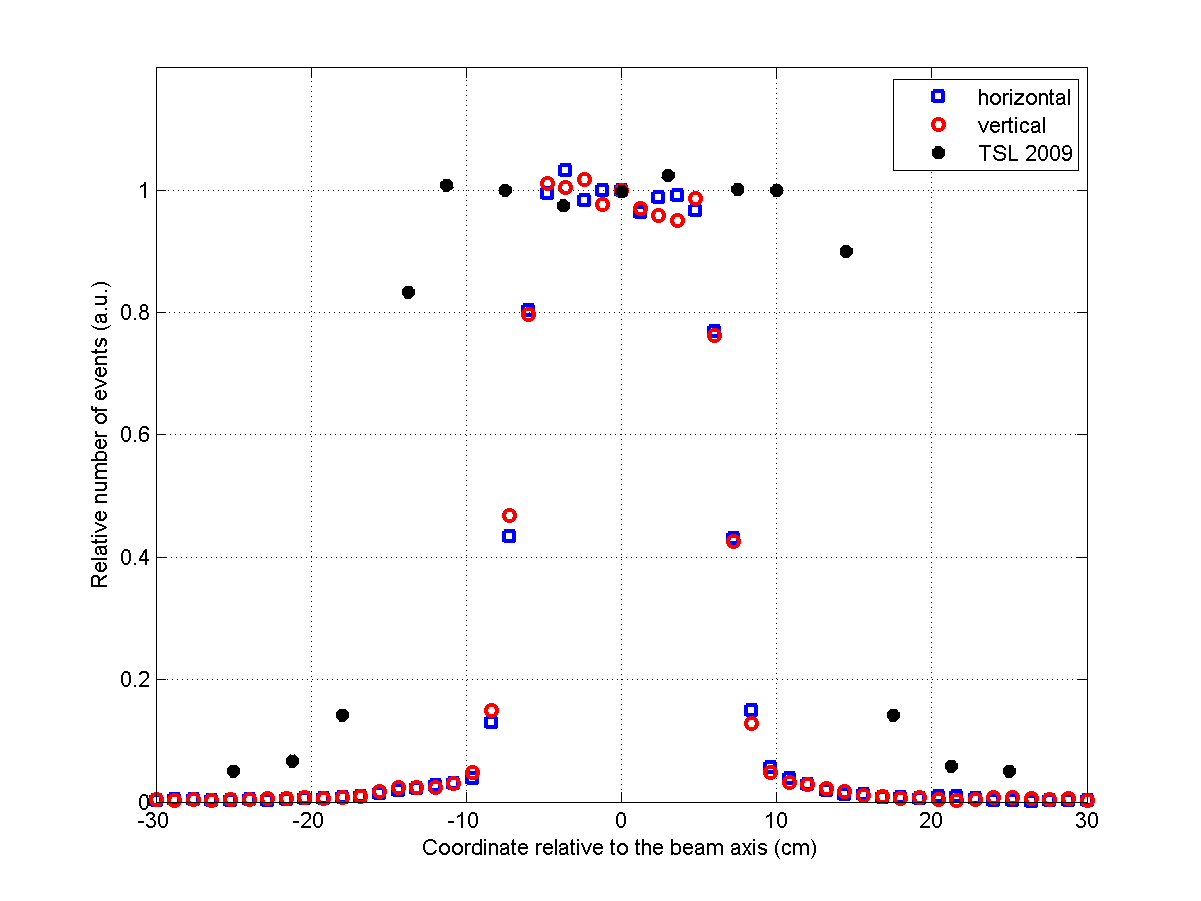
\includegraphics[width=3in]{SUP10beamproFoldingRADECS.png}
% \todo{Show SUP profile, compared to measurements}
    \caption{Neutron profile at the Standard User Position}
    \label{fig:SUPProfile}
\end{figure}

Fig.~\ref{fig:SUPSpectraComparison} compares calculated neutron yield versus energy in the umbra at the SUP with that predicted by the naked-target simulation~\cite{Platt13} and with the standard ANITA SUP parameterisation~\cite{Prokofiev2009}.
The results show\ldots\todo{Discuss the results. Compare current with earlier calculations. Compare calculations with parameterisation.}

\begin{figure}[t]
%    \vspace{2in}
%	\subfloat[Integral fluence rate]{\todo{Integral spectra on log-log axes}\hspace{\columnwidth}}\\
	\subfloat[Integral fluence rate]{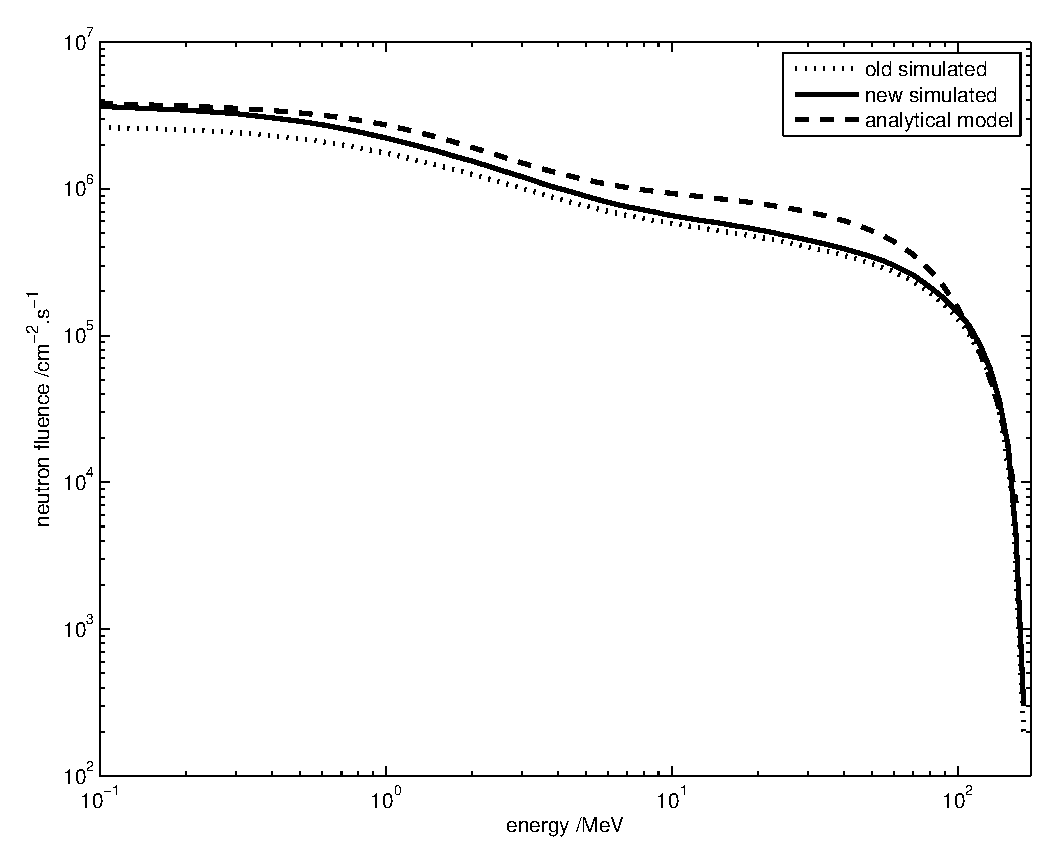
\includegraphics[width=3in]{SUPcomparedIFluxRADECS.eps}\hspace{\columnwidth}}\\
%    \vspace{2in}
%	\subfloat[Equilethargic spectrum, normalised to fluence above \SI{10}{\MeV}]{\todo{Normalised spectra on lethargy axes}\hspace{\columnwidth}}
	\subfloat[Equilethargic spectrum, normalised to fluence above \SI{10}{\MeV}]{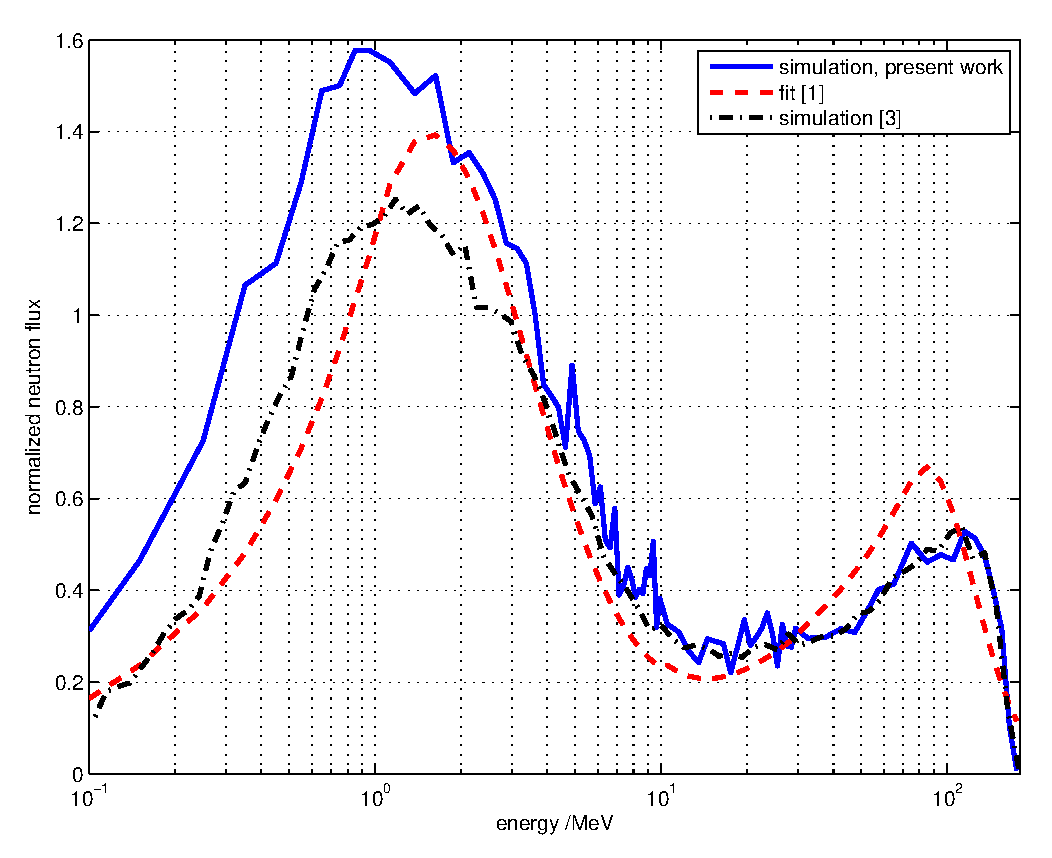
\includegraphics[width=3in]{SUPNormalisedRADECS.eps}\hspace{\columnwidth}}
	\caption{Neuton spectrum at the SUP, showing comparison between the standard facility parameterisation~\cite{Prokofiev2009} and results from a naked Geant4 model~\cite{Platt13} and this work.}
	\label{fig:SUPSpectraComparison}
\end{figure}

Fig.~\ref{fig:CUPDensity} and Fig.~\ref{fig:CUPProfile} show neutron spatial distribution (for neutrons above \SI{10}{\MeV}) and profile (folded in energy with the \U238\ fission cross-section) at the CUP.
The results show\ldots\todo{Describe the results: contours and profile at CUP}

\begin{figure}[t]
%    \vspace{2in}
    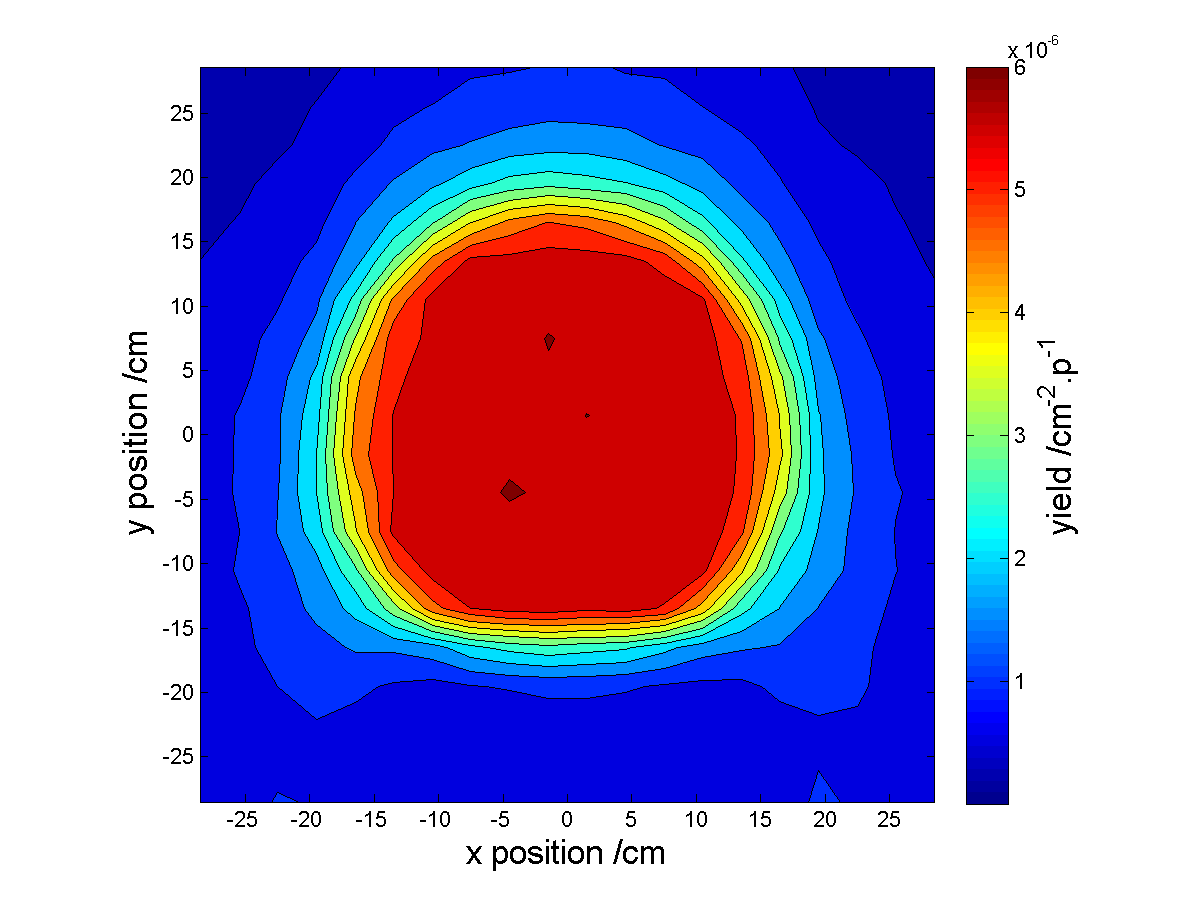
\includegraphics[width=3in]{CUP10ColSpatialDistribution10MeV.png}
% \todo{Show density of neutrons above \SI{10}{\MeV} at CUP}
    \caption{Neutron fluence rate above \SI{10}{\MeV} at the Close User Position.}
    \label{fig:CUPDensity}
\end{figure}

\begin{figure}[t]
%    \vspace{2in}
    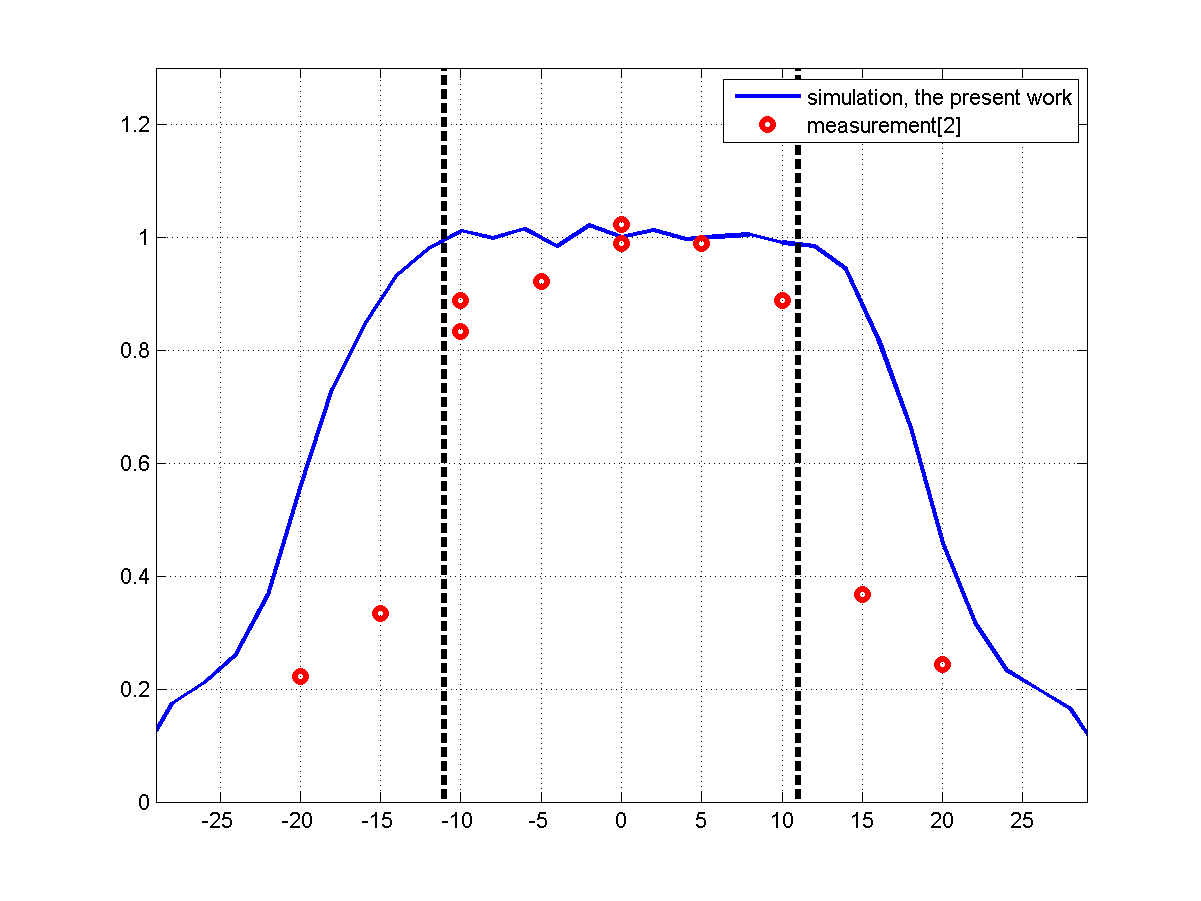
\includegraphics[width=3in]{CUPTOF10beamproRADECS.png}
% \todo{Show CUP profile, compared to measurements}
    \caption{Neutron profile at the Close User Position}
    \label{fig:CUPProfile}
\end{figure}

Fig.~\ref{fig:CUPSpectraCOmparison} compares the spectrum calculated at the CUP with that from the standard parameterisation~\cite{Prokofiev14}.
The latter curve is derived from MCNPX calculations supported by TOF measurements with TFBCs.
The results show\ldots\todo{Explain what the results show: CUP measurement comparison.}
Fig.~\ref{fig:MCComparison} provides a direct comparison between the two Monte Carlo calculations.
The results show\ldots\todo{Explain what the results show (comparison between independent MC calculations).}

\begin{figure}[t]
%    \vspace{2in}
	\subfloat[Integral fluence rate]{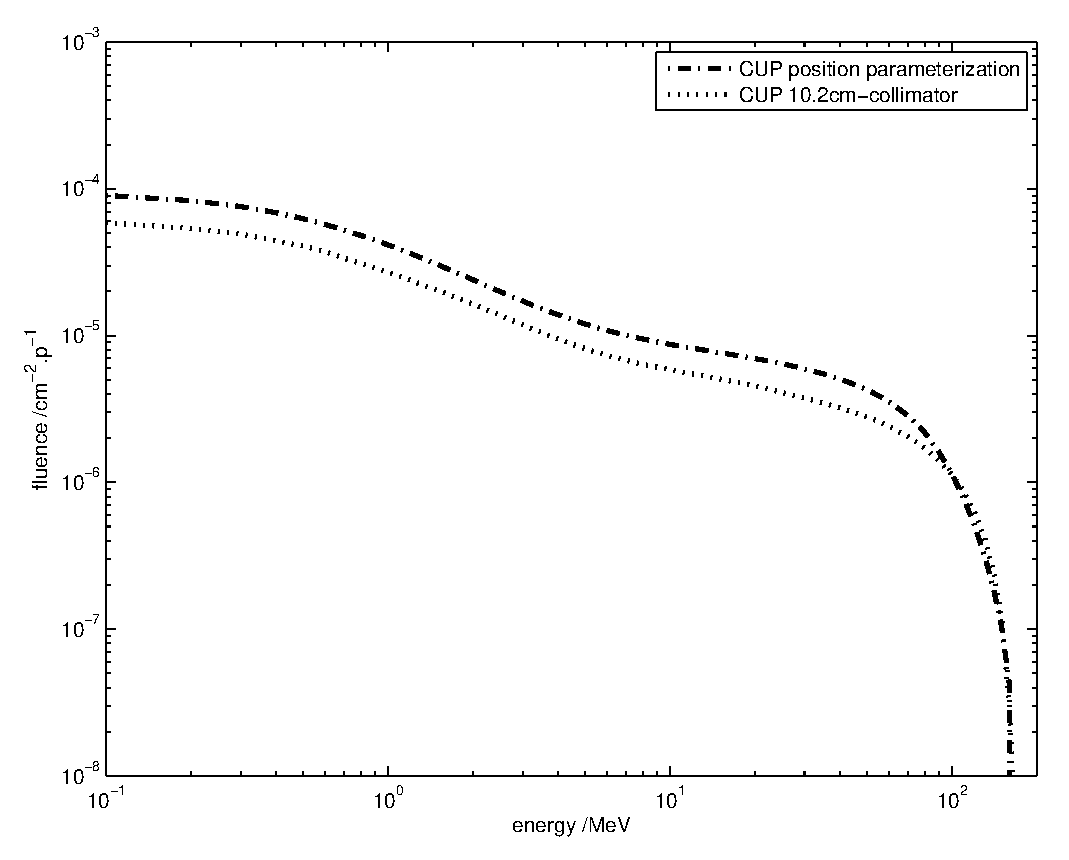
\includegraphics[width=2.5in]{CUPcomparedProkofiev2014linearspaceIFlux.eps}\hspace{\columnwidth}}\\
%    \vspace{2in}
	\subfloat[Equilethargic spectrum, normalised to fluence above \SI{10}{\MeV}]{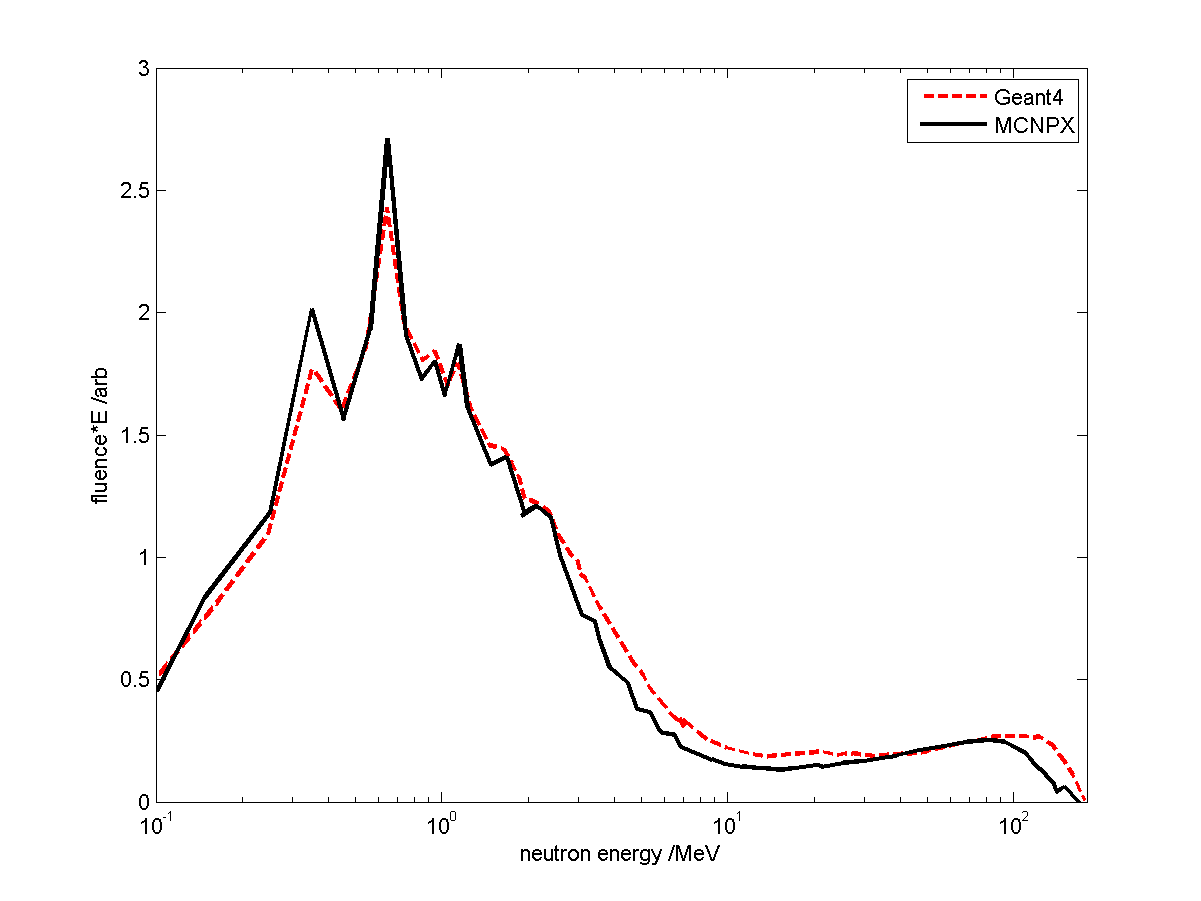
\includegraphics[width=3in]{CUPcomparedLetFluxRADECS.png}\hspace{\columnwidth}}
	\caption{Neuton spectrum at the Close User Position, showing comparison between the standard facility parameterisation~\cite{Prokofiev2009} and results from this work.}
	\label{fig:CUPSpectraComparison}
\end{figure}

\begin{figure}[t]
    \vspace{2in}
    \todo{Show Comparison between Geant4 and MCNPX calculations}
    \caption{Calculated neutron spectra at the CUP-TOF position, compared to independent MCPX calculations~\cite{Prokofiev14}}
    \label{fig:MCComparison}
\end{figure}

Fig.~\ref{fig:DifferentialSpectra} summarise neutron yield results by comparing differential flux as calculated in this work with facility parameterisations~\cite{Prokofiev2009,Prokofiev14}.
The SUP calculations and parameterisations agree very closely below \SI{20}{\MeV}; the parameterisation exceeds the calculations somewhat above that energy.
At CUP the parameterisation exceeds the Geant4 calculations by about TBD\% below \SI{20}{\MeV} and slightly more above that energy.\todo{Improve precision of the summary description of differential spectra.}

\begin{figure}[t]
    \centering
    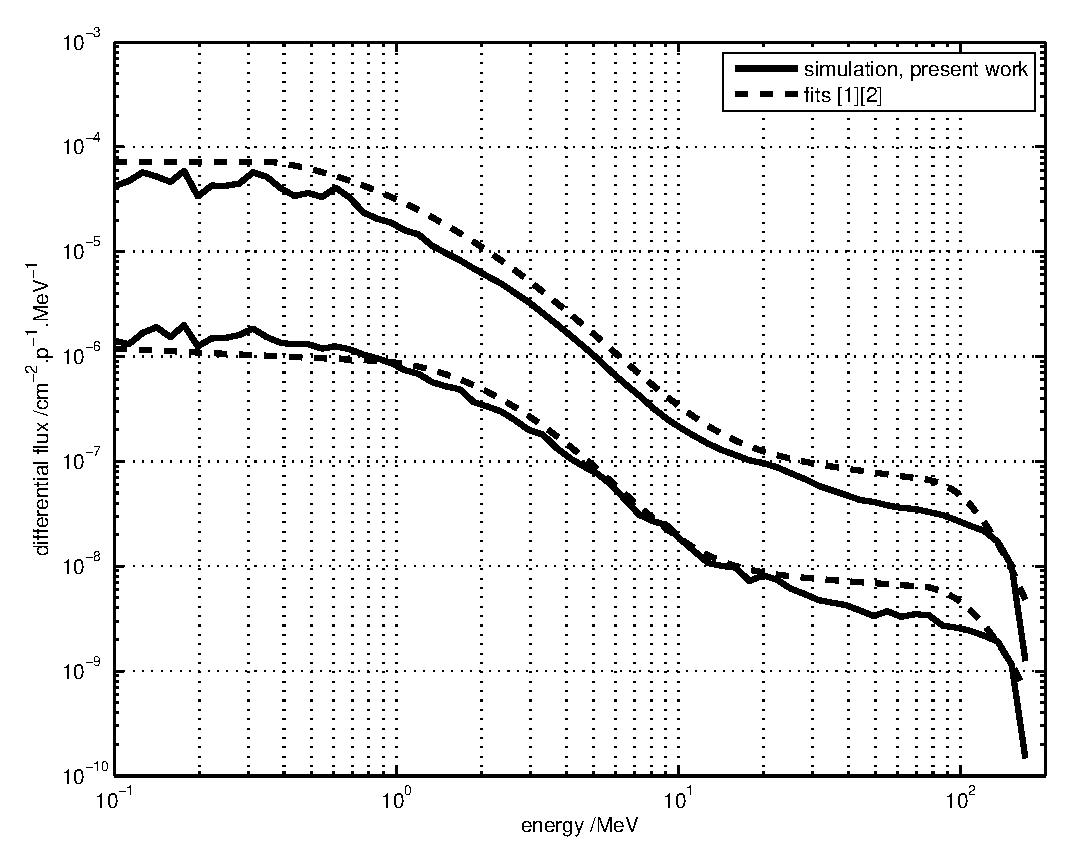
\includegraphics[width=3in]{DiffYieldComparedSUPCUP10.eps}
    \caption{Differential neutron spectra at CUP and SUP, comparing results of this work to facility parameterisations~\cite{Prokofiev2009,Prokofiev14}}
    \label{fig:DifferentialSpectra}
\end{figure}

\subsection{Neutron time of flight}

Neutron beam monitoring and characterisation at TSL uses time-of flight measurements with \U238\ TFBCs.
Our Geant4 model permits these measurements to be simulated.
Neutron time of flight data from the simulation (time measured from the time of arrival of primary photons at the target to the time of arrival of secondary neutrons at the point of interest) were folded in energy with the \U238\ fission cross-section, convolved with a \SI{5}{\ns} rectangle function approximating the primary proton micropulse shape, and overlapped at \SI{45}{\ns}, representing the timing ambiguity due to the micropulse period.
Results are for SUP and CUP-TOF positions and compared with measurements~\cite{Prokofiev2009,Prokofiev14} in Fig.~\ref{fig:TOFSpectra}.
The simulated CUP-TOF results were calculated for the \SI{3}{\cm} collimator, to match the available measured data.
The results show\ldots\todo{Explain what the results show.}

\begin{figure}[!t]
	\centering
	\subfloat[At the CUP-TOF position, with \SI{3}{\cm} collimator]{\todo{Add experimental data to TOF figure (CUP)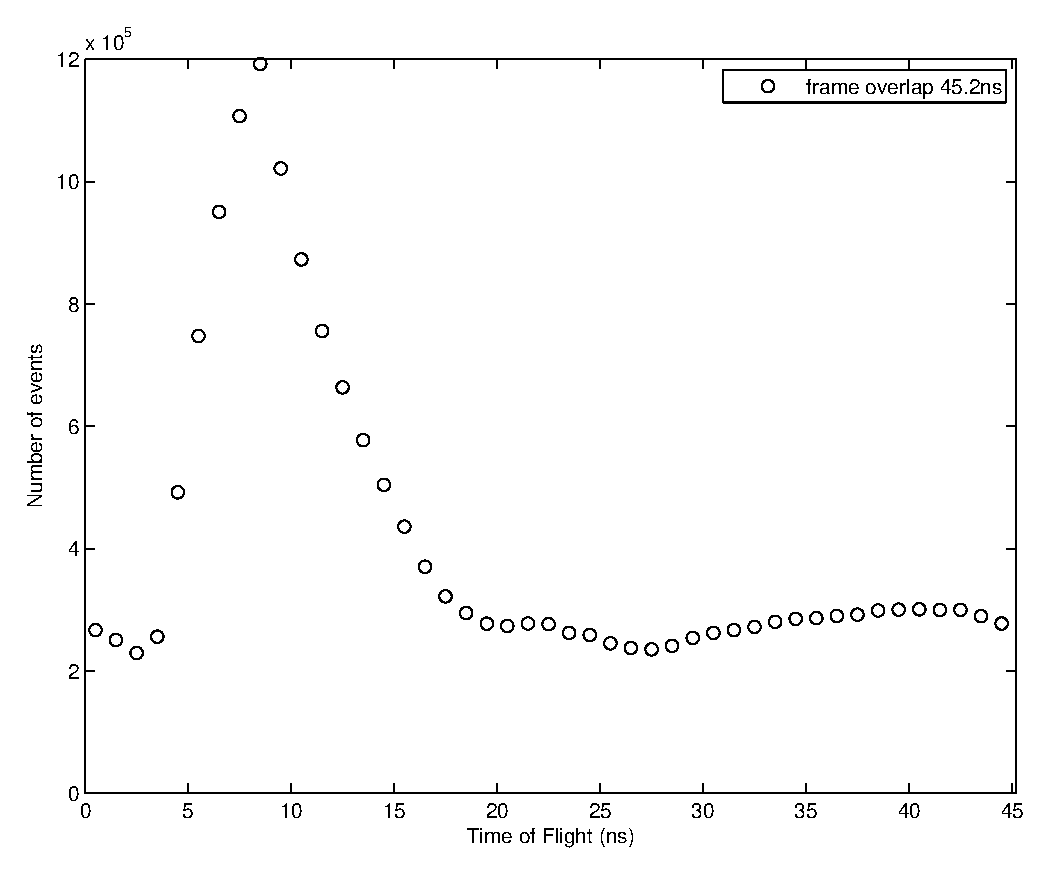
\includegraphics[width=3in]{TOF3frameoverlap.eps}}
	\label{fig:TOFFrameOverlapspectrum}}\\
	\subfloat[At the SUP, with \SI{10.2}{\cm} collimator]{\todo{Add experimental data to TOF figure (SUP)}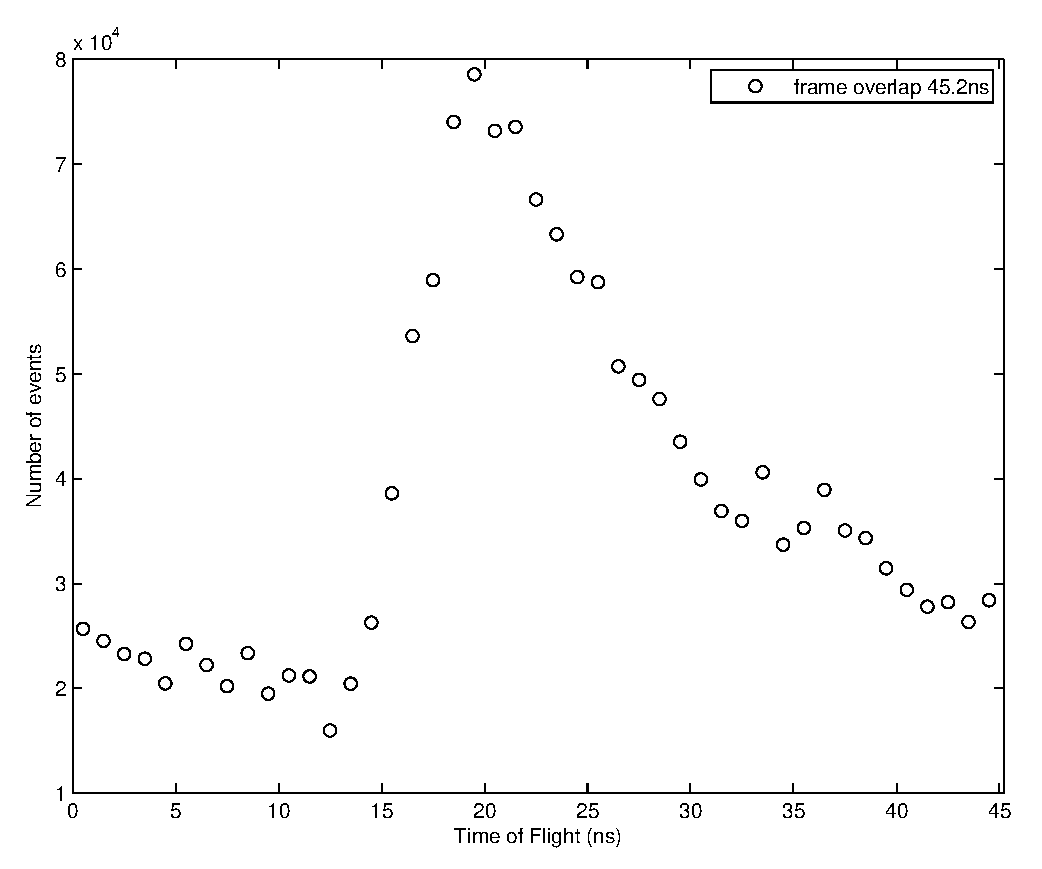
\includegraphics[width=3in]{SUP10frameoverlap.eps}
	\label{fig:SUP10FrameOverlapspectrum}}
    \caption{Simulated neutron time of flight spectra compared to measurements}
    \label{fig:TOFSpectra}
\end{figure}

Prokofiev et at.~\cite{Prokofiev14} explain the TOF spectrum upstream of the collimator as being the resultant of three components: directly from the target, scattered from the target surroundings, and backscattered from the collimator front face.
The complex flight paths and energy losses in the scattered components break the one-to-one relationship between neutron energy and neutron time of flight from target to detector.
We are able to reproduce this situation in our simulation, as shown by Fig.~\ref{fig:TOF3Componentslinear}, which shows good agreement with\ldots\todo{Complete description of the three components.}

\begin{figure}[!t]
	\centering
	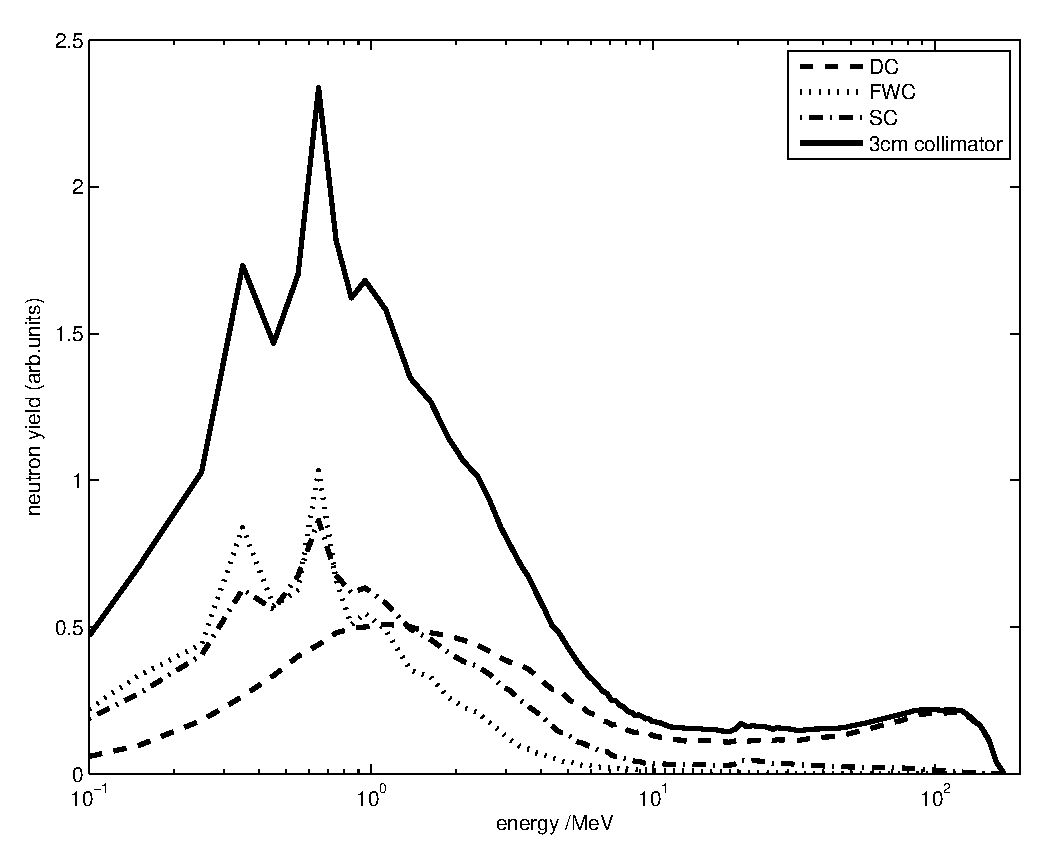
\includegraphics[width=3in]{TOF3Componentslinear.eps}
	\caption{
    Simulated neutron yield with \SI{3}{\cm} collimator at the CUP-TOF position.
    The three components are directly from the target, scattered forward from the target surroundings, and scattered back from the collimator front wall.}
	\label{fig:TOF3Componentslinear}
\end{figure}

\subsection{Gamma fluence rate, spatial distribution and dose rate}

Fig.~\ref{fig:GammaSpatialDistribution} shows the calculated spatial distribution of gamma photons at SUP and CUP.
Fig.~\ref{fig:DifferentialGammaSpectra} shows the calculated differential gamma spectra within the central region of the spatial distribution.
The results show\ldots\todo{Describe the gamma results}

\begin{figure}
    \centering
    \vspace{2in}
    \subfloat[SUP]{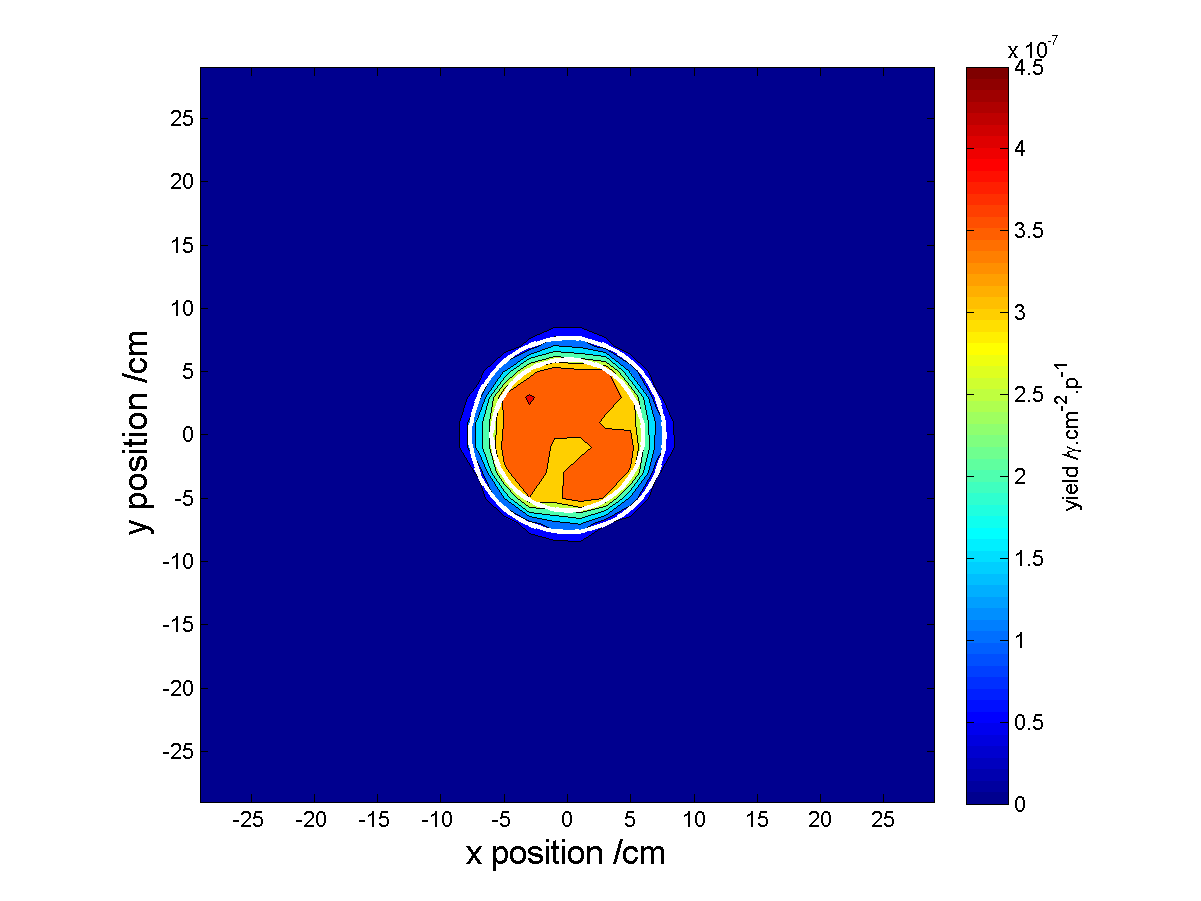
\includegraphics[width=3in]{SUP10ColSpatialDistributionAllG.png}
%     \todo{Add gamma spatial distribution at SUP, \SI{10.2}{\cm} collimator}\hspace{\columnwidth}
        \label{fig:GammaSpatialDistributionSUP}
    }\\
    \subfloat[CUP]{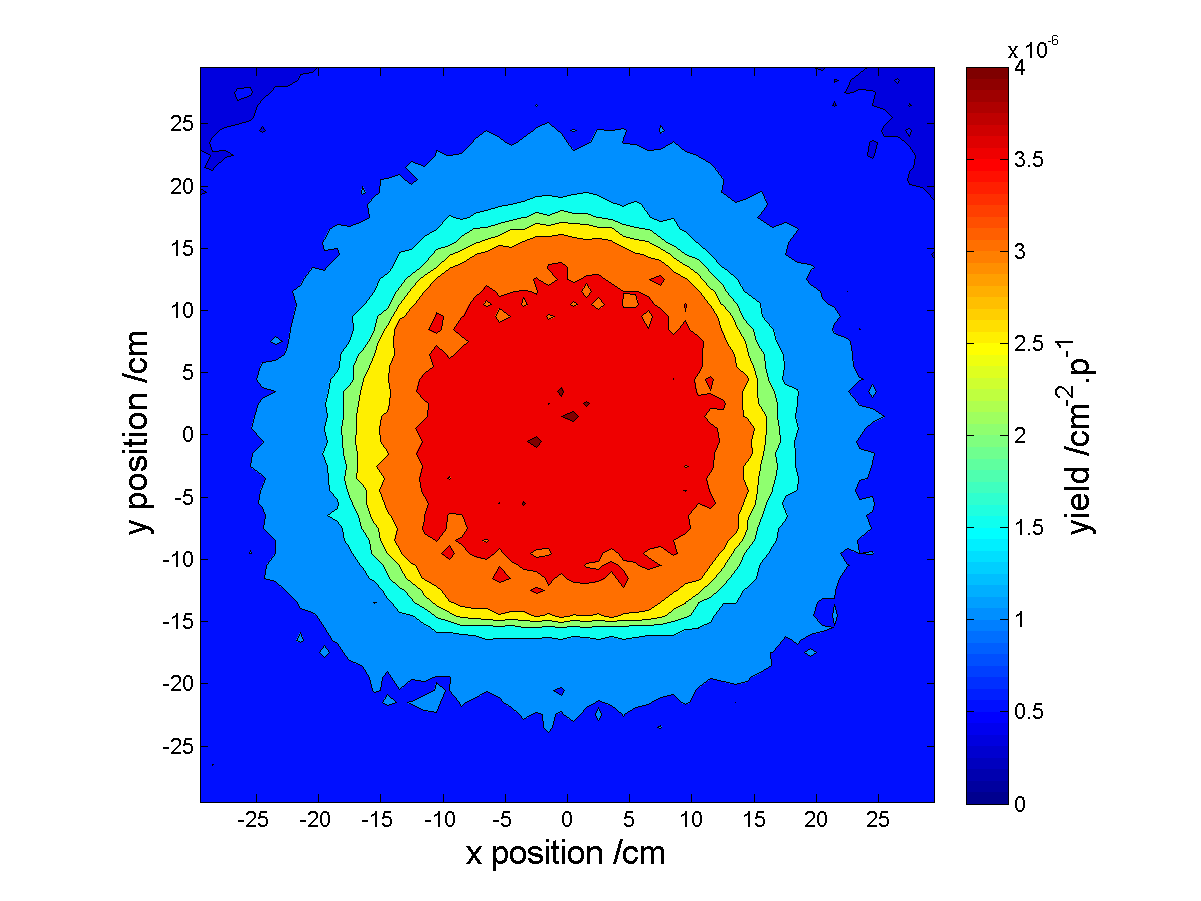
\includegraphics[width=3in]{CUP10ColSpatialDistributionAllG.png}
%     \todo{Add gamma spatial distribution at CUP, \SI{10.2}{\cm} collimator}\hspace{\columnwidth}
        \label{fig:GammaSpatialDistributionCUP}
    }
    \caption{Gamma spatial distribution}
    \todo{It would be better if gamma spatial distribution were expressed as dose, rather than number of photons. Not in time for the abstract submission, however!}
    \label{fig:GammaSpatialDistribution}
\end{figure}

\begin{figure}
    \centering
    \vspace{2in}
    \hspace{\columnwidth}
    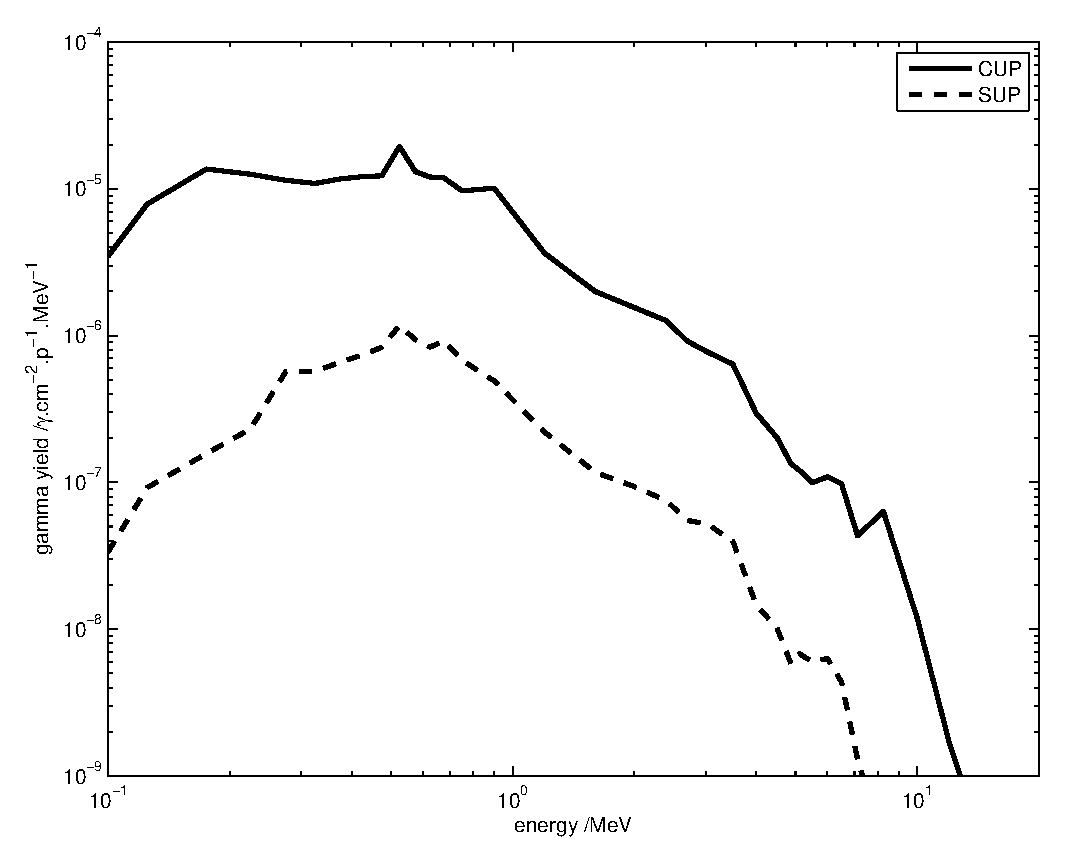
\includegraphics[width=3in]{gDYieldcomparedRADECS.eps}
    \caption{Calculated differential gamma spectra at CUP and SUP}
    \label{fig:DifferentialGammaSpectra}
\end{figure}

Fig.~\ref{fig:GammaDoseEnergy} shows the calculated distribution of gamma dose, obtained by folding the gamma spectra (Fig~\ref{fig:GammaDoseEnergy}) with dose conversion data from \cite{tbd}.
The results show\ldots\todo{Describe the gamma dose versus energy graphs.}
The calculated dose rate at \SI{200}{\nA} primary proton current is \SI{21}{\milli\gray\per\hour} at SUP and \SI{370}{\milli\gray\per\hour} at CUP.\todo{Discuss calculated dose rates}

\begin{figure}
    \centering
    \vspace{2in}
    \subfloat[SUP]{
%	\todo{Add gamma dose versus energy at SUP, \SI{10.2}{\cm} collimator}\hspace{\columnwidth}
        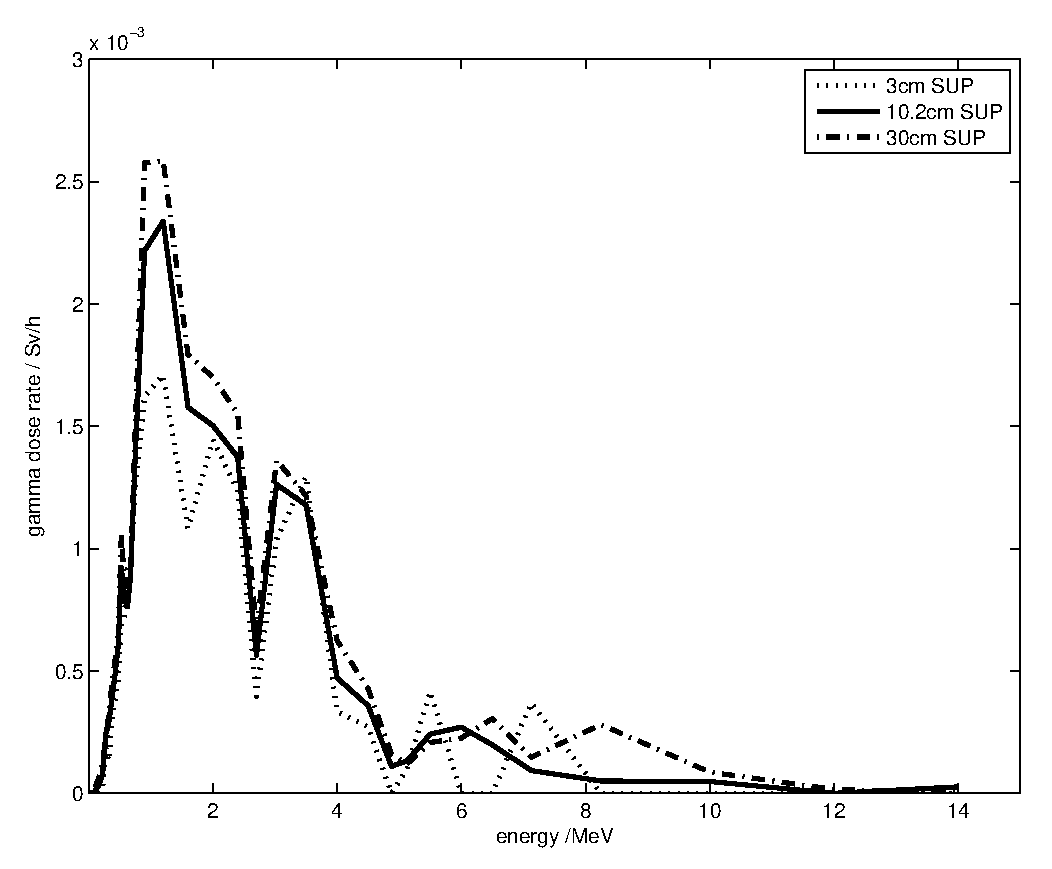
\includegraphics[width=3in]{DoseVSenergySUP.eps}\hspace{\columnwidth}
        \label{fig:GammaDoseEnergySUP}
    }\\
    \subfloat[CUP]{
%     \todo{Add gamma dose versus energy at CUP, \SI{10.2}{\cm} collimator}\hspace{\columnwidth}
        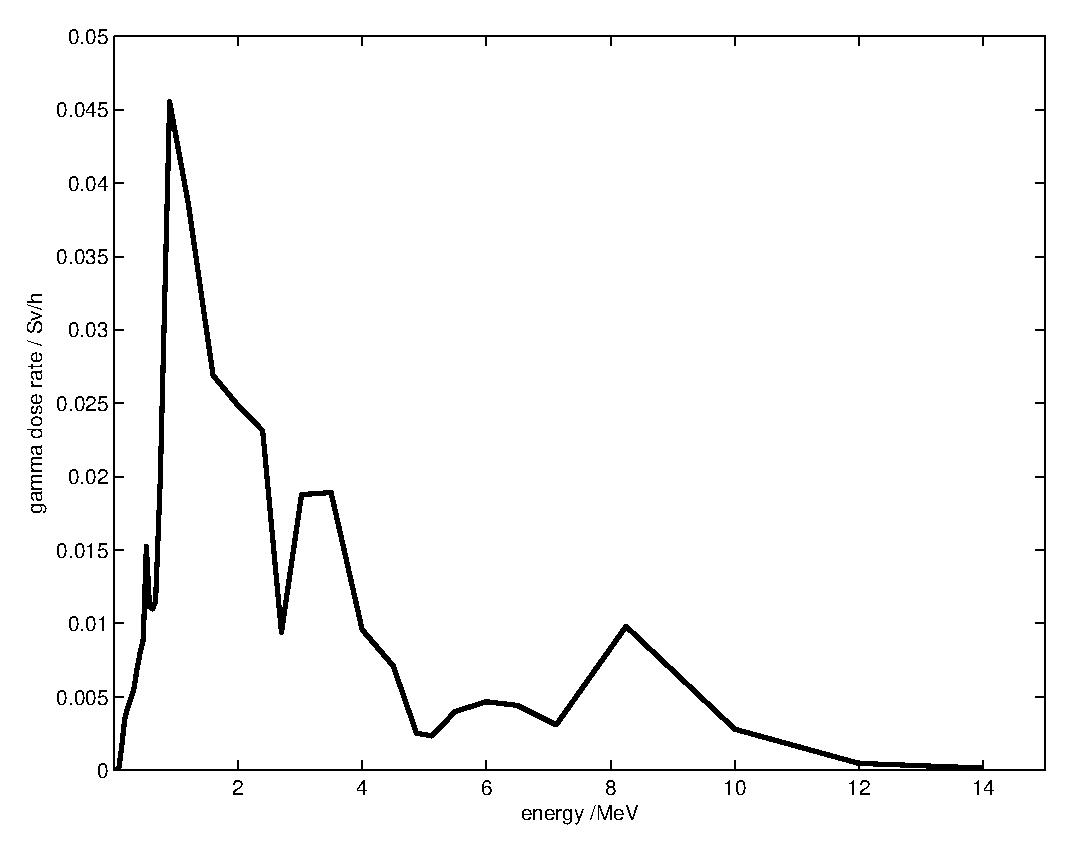
\includegraphics[width=3in]{DoseVSenergyCUP.eps}\hspace{\columnwidth}
        \label{fig:GammaDoseEnergyCUP}
    }
    \caption{Gamma dose spectra}
    \label{fig:GammaDoseEnergy}
\end{figure}


\section{Discussion}
\todo{Discussion}

\ifCLASSOPTIONcaptionsoff
  \newpage
\fi

\todo{Complete citations}

\begin{thebibliography}{99} % Bibliography - this is intentionally simple in this template

\bibitem{Wender87}
S.A. Wender and P.W. Lisowski,
\newblock A white neutron source from 1 to 400 MeV,										% title	
\newblock {\em Nucl. Instr. Meth. Phys. Res. B}, vol. 24-25, pp. 897-900.					% vol:page, 2011

\bibitem{Platt13}
Platt, S.P. and Hong, Q. and Mein, S.J. and Zhang, L.H.,
\newblock Neutron and gamma fields at neutron spallation sources for single-event-effects testing,		% title	
\newblock {\em in Proc. 14th European Conf. Radiat. Effects Compon. Syst. 2013,} pp 1-4			% vol:page, 2011

\bibitem{Prokofiev14}
Prokofiev, A.V. and Blomgren, J. and Majerle, M. and Nolte, R. and Rottger, S. and Platt, S.P. and Cai Xiao Xiao and Smirnov, A.N.,
\newblock Characterization of the ANITA Neutron Source for Accelerated SEE Testing at the Svedberg Laboratory,		% title	
\newblock {\em in Proc. IEEE Radiation Effects Data Workshop. 2009,} pp 166-173 									% vol:page, 2011

\bibitem{Prokofiev2009}
Prokofiev, A.V. and Passoth, E. and Hjalmarsson, A. and Majerle, M.,
\newblock CUP-A New High-Flux Irradiation Position at the ANITA Neutron Facility at TSL,		% title	
\newblock {\em in Proc. IEEE Trans. Nucl. Sci. 2014}, pp 1929-1936 							% vol:page, 2011

\end{thebibliography}

%----------------------------------------------------------------------------------------

\todos

\end{document} 